% Standalone build of the DRIFT system-architecture figure.
% Compiled with: pdflatex architecture.tex
% Then converted to PNG with: pdftoppm -png -r 250 architecture.pdf architecture
\documentclass[border=4pt,tikz]{standalone}
\usepackage{amsmath,amssymb}
\usepackage{tikz}
\usetikzlibrary{positioning,fit,backgrounds,arrows.meta,calc}

\begin{document}

% =====================================================================
% LAYOUT KNOBS — match those in 80_Docu/FinalPaper/main.tex Fig. 1
% =====================================================================
\def\YVision{ 3.0}    % top lane (Core 1 vision pipeline)
\def\YFusion{ 0.9}    % middle lane (Core 1 fusion / output)
\def\YIMU   {-1.2}    % bottom lane (Core 0 IMU pipeline)
\def\HSep   {8mm}     % default horizontal gap between adjacent nodes
\def\XEkf   {8.0}     % absolute X for the EKF block (fusion lane)

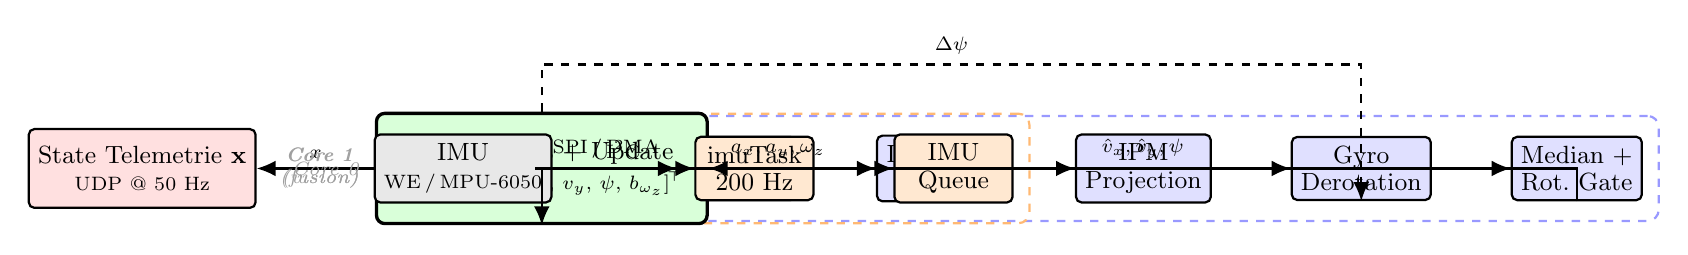
\begin{tikzpicture}[
	>={Latex[length=2.4mm,width=2mm]},
	font=\small,
	every node/.style={align=center},
	hwbox/.style ={rectangle, draw, thick, fill=gray!18,   rounded corners=2pt,
		minimum height=8mm, minimum width=18mm, font=\small},
	visbox/.style={rectangle, draw, thick, fill=blue!12,   rounded corners=2pt,
		minimum height=8mm, minimum width=15mm, font=\small},
	imubox/.style={rectangle, draw, thick, fill=orange!18, rounded corners=2pt,
		minimum height=8mm, minimum width=15mm, font=\small},
	ekfbox/.style={rectangle, draw, very thick, fill=green!15, rounded corners=3pt,
		minimum height=14mm, minimum width=42mm, font=\small},
	outbox/.style={rectangle, draw, thick, fill=red!12,    rounded corners=2pt,
		minimum height=10mm, minimum width=22mm, font=\small}
	]
	
	% --- Core 1 vision pipeline (top row, Y=\YVision) ---------------------
	% Only the first node has an absolute X; the rest chain horizontally.
	\node[hwbox]                          (cam)   at (0, \YVision) {OV3660\\[-1pt]Camera};
	\node[visbox, right=18mm of cam]     (fast)  {FAST-9\\[-1pt]Detector};
	\node[visbox, right=\HSep of fast]    (lk)    {LK Flow\\[-1pt]\scriptsize 7$\times$7};
	\node[visbox, right=\HSep of lk]      (ipm)   {IPM\\[-1pt]Projection};
	\node[visbox, right=\HSep of ipm]     (derot) {Gyro\\[-1pt]Derotation};
	\node[visbox, right=\HSep of derot]   (gate)  {Median +\\[-1pt]Rot.\ Gate};
	
	% --- Core 1 fusion (middle row, Y=\YFusion) ---------------------------
	% EKF anchored at absolute (\XEkf, \YFusion); state node chains right.
	\node[ekfbox]                         (ekf)   at (\XEkf, \YFusion)
	{EKF Predict + Update\\
		\scriptsize $\mathbf{x}=[p_x,\,p_y,\,v_x,\,v_y,\,\psi,\,b_{\omega_z}]^{\!\top}$};
	\node[outbox, left=15mm of ekf]     (state) {State Telemetrie  $\mathbf{x}$\\[-1pt]\scriptsize UDP @ 50~Hz};
	
	% --- Core 0 IMU pipeline (bottom row, Y=\YIMU) ------------------------
	\node[hwbox]                          (imu)     at (0, \YIMU) {IMU\\[-1pt]\scriptsize WE\,/\,MPU-6050};
	\node[imubox, right=18mm of imu]     (imutask) {imuTask\\[-1pt]200~Hz};
	\node[imubox, right=\HSep of imutask] (queue)   {IMU\\[-1pt]Queue};
	
	% --- Vision-row arrows ------------------------------------------------
	\draw[->,thick] (cam)   -- node[above,font=\scriptsize]{SPI\,/\,DMA} (fast);
	\draw[->,thick] (fast)  -- (lk);
	\draw[->,thick] (lk)    -- (ipm);
	\draw[->,thick] (ipm)   -- (derot);
	\draw[->,thick] (derot) -- (gate);
	
	% --- IMU-row arrows ---------------------------------------------------
	\draw[->,thick] (imu)     -- node[above,font=\scriptsize]{I$^{2}$C} (imutask);
	\draw[->,thick] (imutask) -- (queue);
	
	% --- Cross-flow: queue -> EKF (IMU sample drives predict) -------------
	\draw[->,thick] (queue.east) -| node[above,font=\scriptsize,pos=0.25]
	{$a_x,a_y,\omega_z$} (ekf.south);
	
	% --- Cross-flow: vision pipeline output -> EKF update -----------------
	\draw[->,thick] (gate.south) |- node[font=\scriptsize,pos=0.75,above]
	{$\hat{v}_x,\hat{v}_y,\psi$} (ekf.east);
	
	% --- Δψ feedback from EKF state -> derotation -------------------------
	\draw[->,thick,dashed] (ekf.north) -- ++(0,0.6)
	-| node[font=\scriptsize,pos=0.25,above]{$\Delta\psi$} (derot.south);
	
	% --- EKF -> state out -------------------------------------------------
	\draw[->,thick] (ekf.west) |- node[font=\scriptsize,pos=0.75,above]
	{$x$} (state.east);
	
	% --- Lane labels (track the row Y macros automatically) ---------------
	\node[anchor=east, font=\scriptsize\itshape, gray!75] at (-1.2, \YVision) {Core 1\\(vision)};
	\node[anchor=east, font=\scriptsize\itshape, gray!75] at (-1.2, \YFusion) {Core 1\\(fusion)};
	\node[anchor=east, font=\scriptsize\itshape, gray!75] at (-1.2, \YIMU)    {Core 0};
	
	% --- Background grouping boxes ---------------------------------------
	\begin{scope}[on background layer]
		\node[draw=blue!40,   dashed, thick, rounded corners,
		fit=(fast)(gate),  inner xsep=2mm, inner ysep=2.5mm] {};
		\node[draw=orange!55, dashed, thick, rounded corners,
		fit=(imutask)(queue), inner xsep=2mm, inner ysep=2.5mm] {};
	\end{scope}
	
\end{tikzpicture}
\end{document}
